\documentclass[dvipdfmx]{bta}

\title{ハニーポットによる不正ファイルの入手と分析}
\author{G984822019}{吉村 直将}
\supervised{
	\supervisor{教授}{蓑原 隆}
	\supervisor{助手}{田島 信行}
}

%\newenvironment{comment}{\color{red}}{\color{black}}

\begin{document}
\maketitle
\listoffigures

\chapter{はじめに}
%\subsection{研究背景}
% 近年,サイバー攻撃の発生件数が年々増加してきており,その攻撃手法も多様化している.
% 対策として,攻撃者を誘き寄せ,
% 不正アクセスを受けるハニーポットを運用し,
% 攻撃者の情報を収集してきた.過去の研究では,
% ハニーポットを利用して,
% ログイン試行時に使われるIDやパスワード,
% ログイン後に攻撃者から送られるシェルコマンド等の情報を収集し,研究を行ってきた.
% 得られる情報の中でログイン後に送られるコマンドを解析することは、
% 攻撃者がログイン成功後にどうゆう意図で,何を目的をとして攻撃を行なってくるかの予測が立てらる.
% 又,コマンドから攻撃者がダウンロードさせようとしてくる不正なソフトウェアの情報を知り、調査できる為,
% より最新の攻撃に対して具体的なセキュリティ対策につながると思われる.


近年,サイバー攻撃の発生件数が年々増加してきており,その攻撃手法も多様化している.
多様化した新しい攻撃に対処するためには攻撃手法の分析が必要である.
攻撃手法の分析のために,  攻撃者を誘き寄せ,
不正アクセスを受けるハニーポットを用いて
攻撃者の情報を収集
する方法がある.
例えば
ハニーポットを利用して,
ログイン試行時に使われるIDやパスワード,
ログイン後に攻撃者から送られるシェルコマンド等の情報を収集
する方法が提案されている\cite{Entry}.

%ハニーポットは,攻撃を受け,攻撃内容を記録する.その攻撃手法を分析することで,
%攻撃への対策を強化することやデータ収集方法を改良することにつながる.



% 本研究では、ログイン後に攻撃者から送られるコマンドに着目する.
% コマンドについて解析することは、
% 攻撃者がログイン成功後にどうゆう意図を持ち,何を目的をとして攻撃を行なってくるかの予測が立てらる.
% 又,コマンドから攻撃者がダウンロードさせようとしてくる不正なソフトウェアの情報を知り、調査できる為,
% より最新の攻撃に対して具体的なセキュリティ対策につながると思われる.

本研究では,より具体的な攻撃者の攻撃手法の情報を得るため,攻撃者がログイン成功後に行う攻撃に着目し,
ハニーポットを用いて,攻撃者から送信されるコマンドやそのコマンドから入手できるファイルの情報を収集し,解析するシステムを構築する.
そして,攻撃の分析を行い,最新の攻撃内容について警告を発することを目的とする.

\chapter{攻撃収集分析システム}


攻撃者がダウンロードさせようとしてくる
不正なソフトウェアの解析を実現する為のシステムの構成を図\ref{fig:system}に示す.

\begin{figure}[htbp]
	\centering
 	\includegraphics[width=\linewidth]{hpsystem2.png}
 	\caption{システムの構成}\label{fig:system}
\end{figure}


%\subsection{攻撃ホストからハニーポットへの攻撃の流れ}

%攻撃者ホストからハニーポットへの攻撃の流れとして図1に示してある.

% \Repl{攻撃ホスト}{ハニーポット}
% は
% ログイン試行としてID/パスワードを送信してくる
% \Repl{ハニーポットはそれ}{攻撃ホスト}
% に対して,ログイン許可をしている風に見せる.
% \Repl{}{このとき,}ログイン試行時に使われるIDやパスワード
% \Repl{}{を記録する}.

% 攻撃者はログイン\Repl{後}{に成功したシステムを}操作する
% \Repl{為}{ため}に,コマンドを送信する
% \Repl{この攻撃の中でハニーポットはログイン後に}{ので,}
% 攻撃者から送られるシェルコマンド等の情報を収集
% \Repl{し,収集した情報から攻撃手法の研究してきた.}{する}.

ハニーポットは,攻撃者からの何度かのログイン試行を受け,
一定の条件で,攻撃者にログイン成功したと思わせる.
その後,攻撃者にコマンドインタープリタの様な返答を見せ,
不正な操作のコマンドをデータベースDBに収集する.
% 
収集したコマンドから,
攻撃者が不正なサイトから
ダウンロードさせ
ようとする
不正なファイルを安全に入手する.
また,
% コマンドの中には,コマンドからハニーポット内に
% 直接不正なファイルを作成しようとしてくるものもあり,
% 安全にファイルを作成して収集する.
コマンドの中には,ハニーポット内に不正ファイルの作成を試みるものもあり,
安全にファイルを作成し,収集を行う.
% 
収集した不正ファイルのコードから,
どの様な不正ファイルかを分析し警告を発
する.また,
その情報からダウンローダーに生かせるものをフィードバック
する.
% 
% \begin{figure}[htbp]
% 	\centering
% 	\includegraphics[width=\hsize]{honeypot1.png}
% 	\caption{攻撃の流れ}
% \end{figure}

%\subsection{目的}

% 本研究では,ハニーポットDshieldを用いる.DShield(Distributed Intrusion Detection System)は,
% グローバルなセキュリティコミュニティによって構築された分散型侵入検知システムである.
% 世界中のネットワーク上で発生するセキュリティイベントのデータを収集し,
% 分析することでセキュリティの脅威情報を提供する.Dshieldは研究室で以前から運用していたが,
% ログイン試行時のIdやパスワードを収集することを目的としたハニーポットであった.
% 本研究では,ログイン後のコマンドを収集することが目的としている為,
% 新しくハニーポットを構築することとする.                

%\subsection{システムの実装}

本研究では,ハニーポットとしてDShield
(Distributed Intrusion Detection System)\cite{DShield}
と呼ばれるグローバルなセキュリティコミュニティによって構築された分散型侵入検知システム
を使用する.
% 本研究でのハニーポットの実装は,Dshield
% と呼ばれる
% グローバルなセキュリティコミュニティによって構築された分散型侵入検知システム
% をベースに開発を行う.
%世界中のネットワーク上で発生するセキュリティイベントのデータを収集し,
%分析することでセキュリティの脅威情報を提供する.
これまで我々の研究室では主に
攻撃頻度の時系列解析のために
Dshieldハニーポットを利用している\cite{nishida2022}.
が,本研究では図\ref{fig:system}に示すように,Dshieldのcowrie\cite{Cowrie}のログイン認証部,コマンドインターポリタ部に必要な機能を追加する,
また,コマンドからファイル又は,URLなどを取集する
ダウンローダー部,
不正ファイルの分析部は,新しく
プログラムを作成する.
% 研究計画として,
% \begin{enumerate}
%     \item Dshieldを運用できる環境を構築をする.
%     \item コマンドを収集するために、Dshieldのプログラム内で、
% 	攻撃者からのコマンドに対してどのような動作をしているかを確認する.
%     \item 実際にDshieldを運用してみる.
%     \item取集したコマンドの内容について調べる.
%     \item 
%     \item ファイルがどのようなものなのか調べる.
% \end{enumerate}
% という手順で進めていき,攻撃ファイルがどの様なものなのか把握し,
% どのような対策が有効的なのか等の警告を発することで,セキュリティの向上に貢献していく.

%\section{進捗状況}
\chapter{Dshiledの環境構築と運用}

Raspberry PiにDshieldをインストールし,パスワードや接続する無線LANの設定を行なった.
Rassberry Piのファイアウォールの設定からSSHを有効にする事で,
外部からの接続をcowrieが対応するように設定した.
また,研究室内のネットワークからの接続は攻撃と見さないように設定した.

%\subsection{Dshieldが行う攻撃者のログイン試行への対処方法}
設定作業の内容を具体的に記述する.

%Dshieldは研究室で以前から運用されていたがidやパスワードの収集を目的として使われていた.
攻撃者から
コマンドを収集
するために
Dshieldのプログラム
を調査し,
コマンドを収集できているのか確認した.

%まず初めに,Cowrieは,攻撃者からのコマンドをどう対処しているのかを調べ,攻撃者に返すコマンドのディレクトリとしてtxtcomsファイルがあることが分かった.次に,このファイルを使っているものを次のコマンドで検索し,
%\verb!find. -exec grep, 'textcmds' {}\; -and -print 2>/dev/null!
%rv/cowrie/shell/protocol.pyで使われていることが分かった.また,protocol.py内には,getCommand関数があり,この関数はhoneypot.pyでも使われていた.
%srv/cowrie/shell/honeypot.pyで使われていることが分かった.このファイルのLineRacived()関数では,攻撃者が入力された行の処理を行い,その関数内のrunCommand()内のprotocol.getCommand()で実行する.
%また,protocol.py内には,getCommand関数があり,cowrie/src/cowrie/commandsの下にある.pyファイルの中から対応する攻撃コマンドの.pyファイルが実行される.

調査の結果,Dshieldは
Cowrie\cite{Cowrie}を使用して
攻撃コマンドを取集し,
/srv/cowrie/var/log/cowrieの場所にファイル名がcowrie.logやcowrie.jsonに日付が加わった形で保存
していることが分かった.
また,ログイン試行に対応しているプログラムが
/src/cowrie/core/の場所にあるauth.pyである
ことを突き止め,解読したところ,
Dshieldは外部からの攻撃者
%(一つの決まったIPアドレス)
からのログイン試行を1回以上のランダム回数行うと,
ログイン可能とする
ように設定されていることが
分かった.

% そのログイン成功時に使用していた
% ユーザーIDとパスワードがそのIPアドレス限定でのログイン成功するものとなる.
% これは,ハニーポットと見破られないように考えられたシステムだと思われる.

%\subsection{収集したコマンド内容と攻撃者の意図}
実際にハニーポットを運用し5/19から5/30の期間中にコマンドを取集した.
そして,収集したコマンドのファイルデータを扱いやすく,分かりやすくするためのプログラムを作成した.

初めに,コマンド引数でした指定した一つのjsonファイルから一行ずつJsonデータを辞書形式に変更するプログラムとしてreadJson.pyを作成した.また,攻撃者が変わった際に分かりやすいように,ipアドレスが変わったらその都度表示するようにした.
次に複数日のjsonファイルを一括で処理するプログラムをshellスクリプトで作成した.作成したプログラムforList.shは,コマンドで指定したファイル(foo)に書かれているファイルを対象にreadJson.pyを実行する.

\begin{figure}[htbp]

	\lstinputlisting{List/readJson.py}
	\caption{readJson.py}\label{fig:readJson.py}
	
\end{figure}

readJson.pyを図\ref{fig:readJson.py}に示す.
cowrieのJsonデータの方式は,キーと値の形になっている.そこで,6行目でキー['eventid']の値がcowrie.command.inputであることから攻撃者に打たれたコマンド情報であるかの判定を行う.そして,キー['input']の値がコマンドの情報となっている.また,3行目で変数cmdを用意し,今回は,wgetを入れ,12行目で,コマンド情報にwgetに入っているかの判定を行い,求める攻撃コマンドを狭めて確認できるようになっている.

\begin{figure}[htbp]

	\lstinputlisting{List/forList.sh}
	\caption{forList.sh}\label{fig:forList.sh}
	
\end{figure}

\begin{figure}[htbp]

	\lstinputlisting{List/foo}
	\caption{foo}\label{fig:foo}
	
\end{figure}

forLsit.shを図\ref{fig:forList.sh}に,fooファイルを図\ref{fig:foo}に示す.forLsit.shをfooファイル対象として実行した結果を図\ref{fig:forresult}に示す.
\begin{figure}[htbp]

	\centering
 	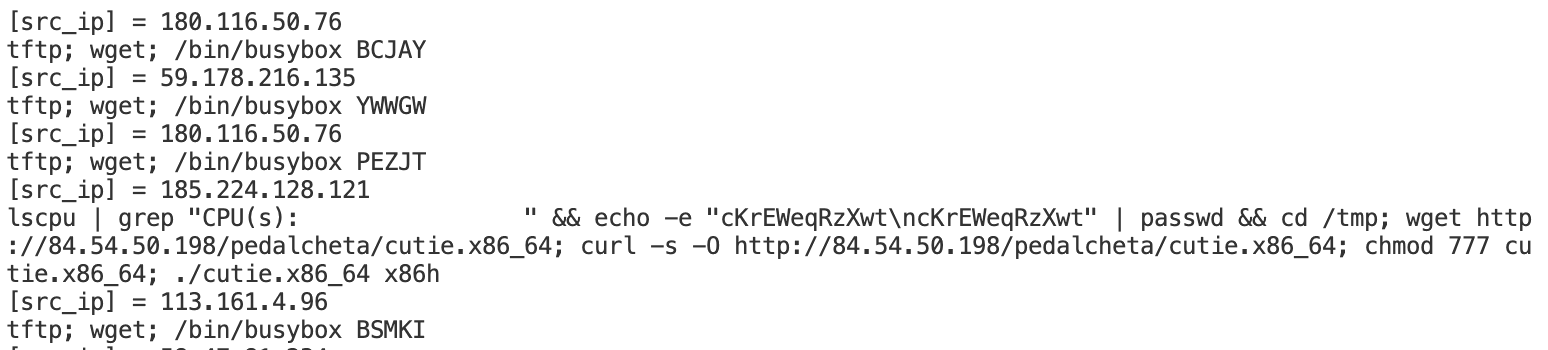
\includegraphics[scale=0.7]{forresult.png}
	\caption{forListの実行結果}\label{fig:forresult}
	
\end{figure}

収集したコマンドの中には,
特定のパターンのコマンドが多く発見された.
例えば組み込みLinuxで複数のコマンドをまとめるために使われる
busyBoxが図\ref{fig:busybox}のように含まれていて,
この期間中に多くの攻撃が組み込みLinuxの機器を対象としていることが分かった.

\begin{figure}[htbp]

	\centering
 	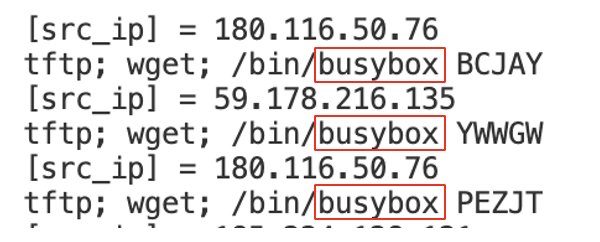
\includegraphics[scale=0.7]{busybox.png}
	\caption{busyboxの攻撃コマンド}\label{fig:busybox}
	
\end{figure}

また,収集したコマンド中には,不正なファイルをダウンロードさせるためwgetコマンドを用いているもの図\ref{fig:wget}や,
不正なファイルをハニーポット内に作成するために,echoコマンドを用いているもの図\ref{fig:echo}が多かった.
\begin{figure}[htbp]

	\centering
 	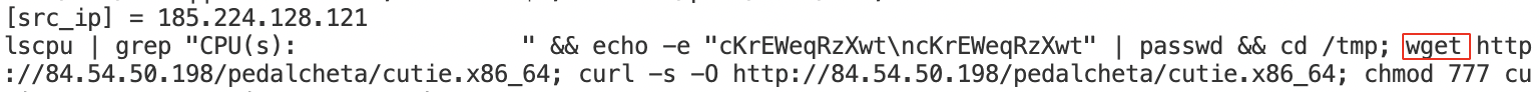
\includegraphics[scale=0.7]{wget.png}
	\caption{wgetの攻撃コマンド}\label{fig:wget}
	
\end{figure}

\begin{figure}[htbp]

	\centering
 	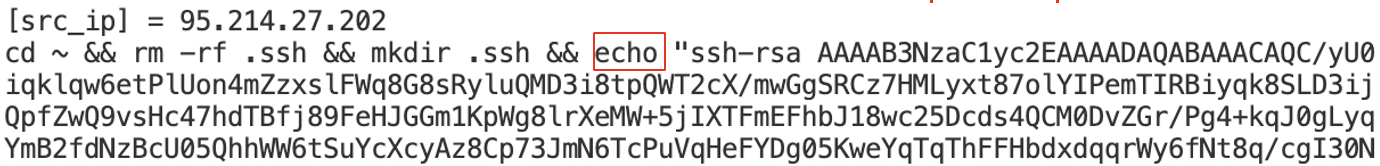
\includegraphics[scale=0.7]{echo.png}
	\caption{echoの攻撃コマンド}\label{fig:echo}
	
\end{figure}

\chapter{ダウンローダー部の作成}
ダウンローダー部のシステムプログラムは,主に3つの動作を行う.

\renewcommand{\labelenumi}{(\arabic{enumi})}
\begin{enumerate}
	\item 不正ファイルデータのダウンロードコマンドを模倣して不正データを入手する
	\item 不正データを安全に扱うためにヘッダ情報を追加する
	\item データを保存するファイル作成し,ヘッダ情報と不正ファイルデータを書き出す.
\end{enumerate}

(1)について,
DshieldがCowrieによって攻撃コマンドを模倣している部分を調査した.
まず初めに,攻撃者に決まった内容の応答を返すコマンドの応答内容が図\ref{fig:textcmds}のようにtxtcmdというディレクトリの下のファイルに置かれていることが分かった.

\begin{figure}[htbp]
	\centering
 	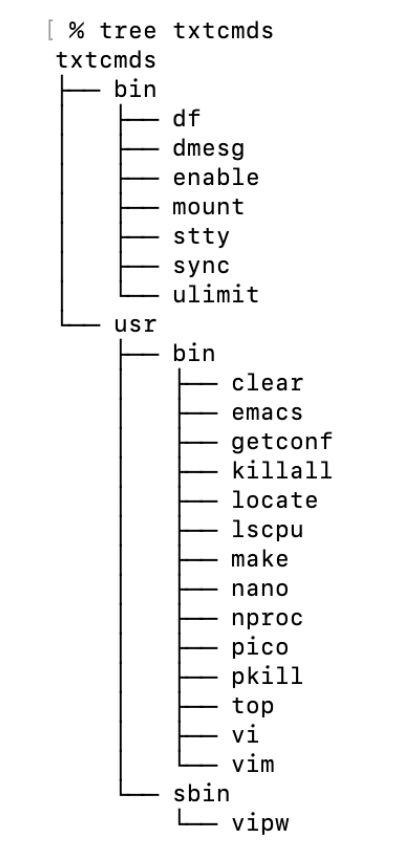
\includegraphics[scale=0.7]{txtcmds.png}
 	\caption{固定的な応答内容のファイル}\label{fig:textcmds}
\end{figure}

次に,このファイルを使っているソースプログラムを次のコマンドで検索し,/srv/cowrie/shell/protocol.py の
getCommand 関数で使われていることが分かった.

\verb!find /srv/cowrie/ -exec grep, ’textcmds’ {}\; -and -print 2>/dev/null!

getCommand関数は/srv/cowrie/shell/honeypot.py で使われており,この honeypot.py の LineReceived 関数で, 攻撃者が入力された行の処理を行うときに,runCommand 関数を呼び出して protocol.getCommand() コマンドを実行して いることがわかった.

さらに,応答が固定的でないコマンドは,srv/cowrie/src/cowrie/commandsの下にPythonプログラムとして実現されていることが分かった.
例えば,不正ファイルデータのダウンロードに使われているwgetの動作は,wget.py中で行われる.

\begin{figure}[htbp]

\lstinputlisting[firstnumber=123]{List/wgetP01.py}
\caption{wgetコマンドのフリをするプログラム(wget.py)の一部}\label{fig:downloader}

\end{figure}

wget.pyの一部を図\ref{fig:downloader}に示す.123行目で
\verb!self.download(self.url, self.outfile)!に引数としてURLとファイル名を渡して,ダウンロードを実行する.

download関数では,twistedライブラリ\cite{Twisted}を使用して,HTTP通信を開始する.
ネットワーク通信に時間が掛かるので,125行目から127行目で,通信終了時に呼び出される関数を登録している.通信が成功したら,\verb!self.deferredaddCallback(self.success)!で登録したsuccess関数が呼び出される.

(2)と(3)の処理についてはwget.pyのsuccess関数にコードを追加して実現した.追加したコードを図4.3に,wget.py全体のリストを付録A.1に示す.



(2)において,
ダウンロードしたデータをそのままファイルとして保存することを避け,不正データのファイルを誤って動作させてしまった場合でも問題が起きないようにする
安全対策のために,ヘッダ情報を不正データに追加する.

具体的なヘッダ情報としては,ダウンロードに使用したURLの前に4桁のURL文字数を追加したものとし,URLの文字数は,4桁の数字を追加したものとする.
%プログラムとしてURLの文字数は,formatメソッドを利用し,0埋めを行う.\verb!hd = '{:04}'.format(hdct)!.

(3)については,
Dshieldハニーポットが攻撃者に見せているファイルシステムの外の領域として外付けHDD(/HD/malwares/tmp/)に作成する,そしてファイル名は,図4.3の234行目のように,MWの後に攻撃があった日時を入れたものとする.

図の236行目から239行目が実際にファイルを書き込む部分である.download関数がダウンロードしたデータは変数に記録されているので,ヘッダの後にその内容を書き出している.

%\verb!fname = "/HD/malwares/tmp/MW" + str(now.date()) + "_" + str(now.time())!,
%open関数でファイルを作成する.\verb!self.file = open(fname, "wb")!.
%Dshieldハニーポットが攻撃者に見せているファイルシステムの外の領域に,攻撃があった日時を追加した名前のファイルを作成する.

実際に研究室で運用しているハニーポットに組み込んで確認したところ,攻撃があったときにデータが記録されていないことが判明した.原因はDShieldが1日に1回,18時28分に,配布元を確認し,システムのアップデートがあった時,自動的に更新しているためであった.自動更新が行われると,修正したwget.pyが上書きされてしまい,追加した処理が行われていなかった.

そこでハニーポットの/etc/cron.d/dshieldに変更を加え,アップデートが終了したあとで,wget.pyへ周期的に変更を加えたもので上書きをするように設定し,正しく動作していることを確認した.

\chapter{不正ファイルの分析}
不正ファイルの分析として実際の不正ファイルからの情報取得を行った.
具体的には,直接不正ファイルを作成させようとしてくる攻撃の 1 つとして,
複数の echo コマンド を次のように送るものについて,実際にファイルを作成して調査した.

\verb!echo -ne "\x7f\x45.." > niggabox!

以下,作成したファイルを対象データと呼び. その先頭部分を図\ref{fig:textcmds}に示す.

\begin{figure}[htbp]
	\centering
 	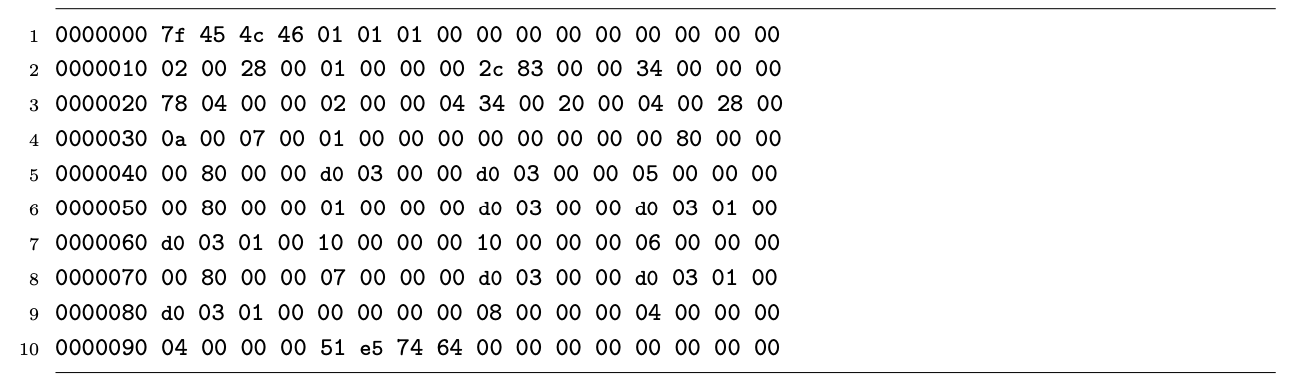
\includegraphics[scale = 0.75]{niggabox.png}
 	\caption{対象データの先頭部分}\label{fig:textcmds}
\end{figure}
まず,対象データは2,720バイトのバイナリーデータであることがわかった.
バイナリーデータのファイルは,最初の数バイトがファイル形式を示している場合が多い.対象データについて先頭部分を調べたところ,
最初の4バイトが,“7f 45 4c 46” であり,ELF形式\cite{elf}のファイルであると判別した.

次にELF形式のヘッダ情報の解析を行う.ELF形式のファイル構造では,

\begin{itemize}
	\item 1から4バイト目がマジックナンバーとして"7f 45 4c 46"に固定されている
	\item 5バイト目がクラスとして,32ビットオブジェクト(1)か,64ビットオブジェクト(2)かを示している
	\item 6バイト目がデータの符号化として,リトルエンディアン方式(1)かビックエンディアン方式(2)かを示している
	\item 18バイト目が対象としているアーキテクチャの種類(28はARM)を示している
	
  \end{itemize}

今回の対象データは,32ビットのリトルエンディアン形式で,ARMアーキテクチャ用であることがわかる.

そこで,次のコマンドで逆アセンブリを行い内容を確認したところ,

\verb! objdump --print-imm-hex!
--disassemble -s niggabox!

マルウェアのMiraiのソースコード\cite{Mirai}として公開されているコードの一部に酷似していることがわかった.

さらに,リンク先から別のファイルをダウンロードする機能を持っていることが分かり.具体的にこの不正ファイルでは,リンク先はアムステルダムで,別のファイルはjklarm7というファイルであることも分かった.


%不正ファイルの分析に伴い,初めに実際の不正ファイルから具体的に何の情報が得られるかを調べた.
%まず,直接不正ファイルを作成させようとしてくる攻撃コマンドの1つである echo -ne "\x7f\x45.." > niggabox を
%利用し,そこから得られる不正ファイルデータから調べた.
%ファイルのバイナリーデータは,最初の数バイトがファイル形式を示している.
%その為,最初の数バイトでファイル形式を判別する.
%今回得られた不正ファイルデータの一つは,最初の4バイトが"x7f x45 x4c x46”であることから,
%ELF形式のファイルであると判別できた.
%また,ファイル形式の種類によって構造は主に決まっていることから,
%その形式の構造からファイルの情報を取得できる.
%よって,ELF形式のファイル構造を調査する.

\section{ELF形式のファイルから情報取得の自動化}
ELF形式のファイルについて,自動で情報を解析するためのプログラムを作成した.

ELF形式は図\ref{fig:elf}に示すように,
ELFヘッダ(ELF Header)につづくデータ部分になっており,データ部分は,プログラムヘッダテーブル(Program header table)または,セクションヘッダテーブル (Section header table) の情報にしたがって,
実行時にメモリ上に展開される.text,.rodataなどの複数セクションで構成されている.

プログラムヘッダテーブルとセクションヘッダテーブルのサイズやオフセットの情報は,ELFヘッダから取得できる.また,各セクションの境界はセクションヘッダの情報で切り分けられる.セクションヘッダテーブルは,エントリという項目で分かれており,各エントリは一つ一つのセクションの情報について書かれている.

\begin{figure}[htbp]
	\centering
 	\includegraphics[width=0.5\linewidth]{elf.png}
 	\caption{ELF形式のファイル構造}\label{fig:elf}
\end{figure}

自動情報取得として,プログラムに埋め込まれた文字列などのリテラルが格納されている.rodataから情報を取得する処理をするプログラムelf.pyを実装した.
elf.pyは,図\ref{fig:elf.py}に示す.
\begin{figure}[htbp]

	\lstinputlisting{List/elf.py}
	\caption{elf.py}\label{fig:elf.py}
	
\end{figure}

elf.pyでは,初めに4行目でELF形式のファイルであるか判別する.次に,6行目から28行目で手作業での分析の際に取得したファイルの基本情報をファイルのヘッダテーブルから取得する.その基本情報を元に,データを,struckモジュールのunpackを使用して,データ方式にのとった方法で変換していく.例えば,24行目,verb!e1 = struct.unpack("<lll",data[24:24+12])!では,ファイルデータの24バイト目から12バイト分のデータを4バイトずつリトルエンディアン方式で,e1として取得する.24行目から45行目まで,他2つのヘッダである,プログラムヘッダーテーブルやセクションヘッダテーブルのオフセットやサイズを取得している.その中の44行目に,.shstrtabというセクションのインデックスの情報としてshstrndxがある.ELF形式では各セクションが記録される順番は規定されていないが,.shstrtabは,各セクション名のテーブルが格納されたセクションであることから,セクションの判別を行うことができる.
次に,51行目から54行目で,セクションヘッダテーブルのセクションごとのデータのリスト(sehd)として,取得したオフセットやサイズ情報を元に,データをunpackし,リストに追加していった.
このセクションヘッダテーブルのリストから,59行目で,shstrndxを利用し,.shstrtabのセクションのオフセットは,sehd[shstrndx][4],サイズは,sehd[shstrndx][5]であるとセクションヘッダテーブルのエントリの項目から確認でき,.shstrtabのデータをshstrとして取得した.
63行目72行目で,セクションヘッダテーブルのエントリの最初の項目では,.shstrtabの対応するセクション名のオフセット情報を持つことから,セクション名snameを取得していった.その際に74,75行目でセクション名.rodataかを判定し,.rodataのエントリのインデックスとしてrdenを取得することで,.rodataのセクション内容を取得するように実装した.

%ELF形式では各セクションが記録される順番は規定されていないが,各セクションの名前のテーブルが格納されたセクション(.shstrtab)があり,ELFヘッダから取得できる.
%elf.pyでは,初めに4行目でELF形式のファイルであるか判別し,6から28行目で手作業での分析の際に取得したファイルの基本情報を取得する.その基本情報を元に,
%各エントリ内の一部が.shstrtabセクションのテーブルの番号の情報をもつため,その番号で各エントリがどのセクションかを判断ができる,そこで,.rodataを検索し,対応するセクションの内容をダンプするようなプログラムとしてelf.pyを作成した.




手作業での分析に使用した対象データ(niggabox)について,作成したプログラムを実行し,図\ref{fig:jklarm7}のようにダウンロードしようとするファイル名(jklarm7)などの情報が取得できることを確認した.


\begin{figure}[htbp]
	\centering
 	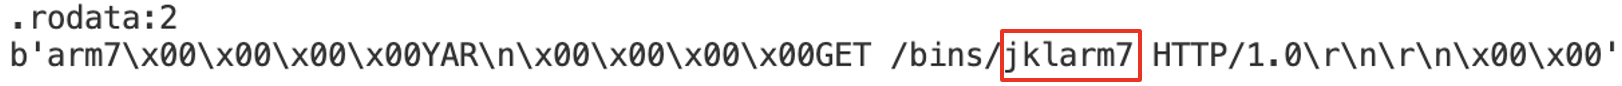
\includegraphics[scale = 0.6]
	{jklarm7.png}
 	\caption{ELF形式データからの情報抽出結果}\label{fig:jklarm7}
\end{figure}

%ELF形式のファイル構造は,複数のセクションから構成されている.
%その中に3つのヘッダとして,ELFヘッダ,プログラムヘッダ,セクションヘッダがあり,
%主にヘッダは各セクションについての情報を持っている.
%ELFヘッダは,他2つのヘッダ情報を持っており,大きさや位置情報が取得できる.
%また,セクションヘッダでは,各セクションごとに何の情報を持っているか等が分かる.
%その為,この二つのヘッダを利用して,どういった情報を持っているかの判別を行う.
%また,セクションヘッダ内は,エントリという項目で分かれていて.
%各エントリは,セクション一つ一つに対応して,
%そのセクションがどういったプログラムやデータかや,サイズやオフセット等の情報を持っている
%また,セクションの一つに,各セクションの名前が羅列された.shstrtabがある.
%こののセクションを利用し,各エントリが
%.shstrtab内にあるセクション名への位置情報を持っていることから、
%対応付けし,各セクションの名前を知ることができる.
%このような形でelf形式の構造からどういったファイル情報を取得すること可能かが分かった.

\chapter{まとめ}

本研究では,Dshieldハニーポットに,ダウンローダー部や解析を行うプログラムelf.pyなどの機能を追加することで,
ダウンローダー部では攻撃コマンドが送り込もうとしている不正ファイルデータを取得し,
elf.pyではELF形式のファイルの解析を行うシステムの開発を行なった.
そして,我々の研究室で運用しているハニーポットに実装した,
運用をしていきながら攻撃データを収集していった結果,
収集した攻撃コマンドは,wgetやechoのようなコマンドが確認でき,
その攻撃コマンドを利用し,ダウンローダー部で不正ファイルデータの取得を行い,次に,解析結果の表示を行えることを確認した.
具体的な解析結果として,攻撃コマンドechoから取得した不正ファイルデータの一つがMiraiと呼ばれるマルウェアに酷似しており,リンク先であるアムステルダムから別のファイルjklarm7をダウンロードする機能を持っていることが分かった.
しかし,解析結果を管理者に通知する部分は未実装で残された課題となっている.

%\bibliographystyle{entry}
\bibliographystyle{ipsjunsrt}
\bibliography{sample}

\appendix

\chapter{プログラムリスト}

\lstinputlisting{List/wget.py}
\end{document}
